
\chapter{Diagrammi di Bode}
\section{Rappresentazione della funzione di trasferimento}

%TODO: Io la riscrivo, ma forse è meglio fare riferimento al capitolo 3 e magari metterci un link sul capitolo 3 e sottolineare la formula della funzione di trasferimento

%TODO: inserire una riga d'intestazione per non fare iniziare la sezione con una formula centrale

\begin{equation}
	H(j\omega) \dot{=}\int_{-\infty}^{+\infty} \! h(t)e^{-j\omega t} \d t
\end{equation}
dato uno specifico $\omega$ abbiamo un risultato nel piano complesso:
\[
	H(j\omega) \big\vert_{\omega = \omega_k}
\]

%TODO non so dove piazzare questo diagramma nel contesto
%TODO: fare immagine
%\begin{figure}[H]
%	\centering
%	\includegraphics[width=0.7\linewidth]{immagini/cap6_Bode/diagNyquist}
%	\caption{ Diagramma di nyquist: la funzione di trasferimento viene rappresentata come una curva parametrica al variare di $\omega$.  }
%	\label{fig:diagNyquist}
%\end{figure}

La rappresentazione su grafici rende più facile l'interpretazione della funzione di trasferimento. Per semplicità si può dividere il segnale nel modulo e nella fase.


\begin{align}
 A(\omega)&=\abs{H(j\omega)}=\Abs{\int_{-\infty}^{+\infty} \! h(t)e^{-j\omega t} \d t} &\text{funzione pari}\\	
 \Phi (\omega)&= \arg(H(j\omega)) & \text{funzione dispari}
\end{align}


Rappresentiamo un numero complesso $z=a+jb$

\begin{figure}[H]
	\centering
	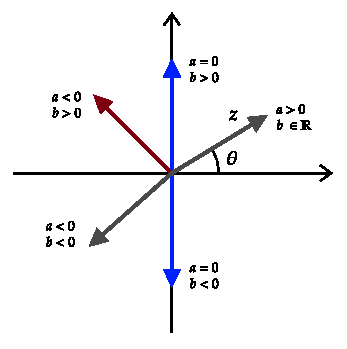
\includegraphics[width=0.4\linewidth, valign=c]{immagini/cap6_Bode/argCompl.pdf}\quad
	$ \displaystyle \arg(z) =
	\begin{cases}
		\arctan \big(\frac{b}{a}\big) &a>0, b\in \R\\
		\frac{\pi}{2}&a=0, b>0\\
		-\frac{\pi}{2}&a=0, b<0\\
		\arctan \big(\frac{b}{a}\big)+\pi &a<0, b\ge 0\\
		\arctan \big(\frac{b}{a}\big)-\pi &a<0, b< 0
	\end{cases} $
\end{figure}

Vista l'ampiezza delle possibili frequenze, usualmente si usa una \textbf{scala logaritmica} per esse. Vediamo come usare il logaritmo nei numeri complessi.

Nei reali: 
\begin{equation*}
	y=\ln (x) \iff x e^y, \quad x \in \R, y \in \R 
\end{equation*}
Nei complessi: %TODO da risistemare
\begin{gather*}
	w = \ln (z) \iff z=e^w \quad z \in \C^*, w \in \C \\
	z=\rho e^{j \theta} \quad w=u+jv\\
	z= \rho e^{j \theta} = e^w=e^{u+jv} = e^u e^{jv}\\
	\rho = e^u \rightarrow u = \ln(\rho) \rightarrow u =\ln(\abs{z})\\
	e^{j\theta} = e^{jv} \rightarrow v = \theta \rightarrow v= \arg (z)\\
	\ln (z) = w = u+jv = \ln (\abs{z}) + j \arg (z)
\end{gather*}

%TODO eh?
Logaritmo principale: dove $ -\pi < \arg (z) < \pi $ (oppure $ 0< \arg (x) <2\pi $)

\subsubsection{Proprietà del logaritmo}
\begin{enumerate}
	\item $ \ln ( b c) = \ln (b) + \ln (c) $
	\item $ \ln \Big(\frac{b}{c}\Big) = \ln (b) - \ln (c) $
	\item $ \ln (b^c) = c \ln (b) \quad ,c \in \R$
	\item $ \log_a (b)  = \frac{\log_c (b)}{\log_c (a)}=\underbrace{\frac{1}{\log_c (a)}}_{\text{Costante}}\log_c (b)$
\end{enumerate}

Per analogia:
\begin{enumerate}
	\item $ \arg ( b c) = \arg (b) + \arg (c) $
	\item $ \arg \Big(\frac{b}{c}\Big) = \arg (b) - \arg (c) $
	\item $ \arg (b^c) = c \arg (b) \quad ,c \in \R$
	\item Non c'è cambio di base
\end{enumerate}

\subsection{Decibel}
L'unità di misura dell'ampiezza nei diagrammi di Bode è il Decibel
\[
\abs{H(j\omega)}_{dB} = 20 \log_{10}\abs{H(j\omega)}
\]

%TODO nemmeno qui non so dove piazzare questo diagramma nel contesto
%TODO: fare immagine
%\begin{figure}[H]
%	\centering
%	\includegraphics[width=0.7\linewidth]{immagini/cap6_Bode/diagNichols}
%	\caption{ Rappresentazione logaritmica nel Diagramma di Nichols  }
%	\label{fig:diagNichols}
%\end{figure}

\section{Diagrammi di Bode}
%TODO: fare immagine
\begin{figure}[H]
	\centering
	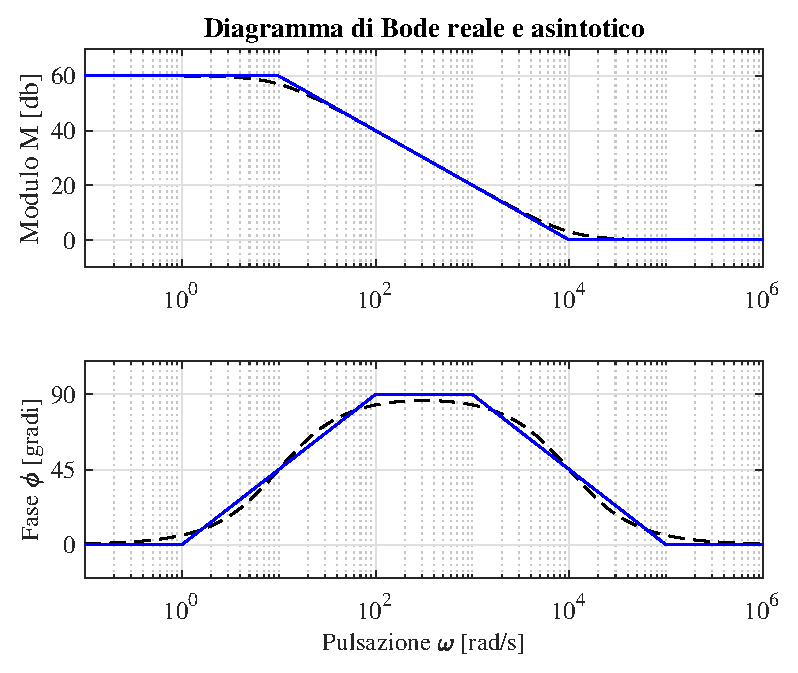
\includegraphics[width=0.7\linewidth]{immagini/cap6_Bode/diagBode.eps}
	\label{fig:diagBode}
\end{figure}

%TODO introduzione migliore da fare

%TODO non so come introdurre i diseng sulle decadi
\begin{figure}[H]
	\centering
	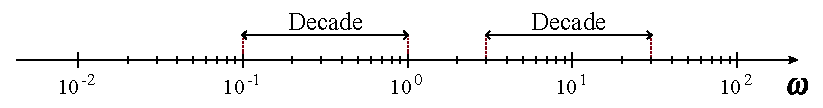
\includegraphics[width=0.7\linewidth]{immagini/cap6_Bode/decade.pdf}
	\label{fig:schDecade}
\end{figure}
Considerando un punto nella decade tra $ 0 $ e $ 1 $ specifichaimo per gli esercizi
\[ 
	\log 2 \simeq 0,3 \quad \log 3 \simeq 0,5 \quad\log 5 \simeq 0,7 \quad\log 8 \simeq 0,9 
 \]
%\begin{figure}[H]
%	\centering
%	\includegraphics[width=0.7\linewidth]{immagini/cap6_Bode/schDecade2}
%	\label{fig:schDecade2}
%\end{figure}
Con l'insieme dei due diagrammi di Bode (diagramma delle ampiezze e diagramma della fase) si ha una rappresentazione logaritmica di $ H(j\omega) $
\[ 
	\ln \big(H(j\omega)\big) = \underbrace{\ln (A(\omega))}_{\text{diagramma Ampiezze}} + j\,\underbrace{\Phi (\omega)}_{\text{diagramma Fase}}
 \]
 
 In caso di un sistema:
% \begin{figure}[H]
% 	\centering
% 	\includegraphics[width=0.7\linewidth]{immagini/cap6_Bode/sist1}
% 	\label{fig:sist1}
% \end{figure}
\begin{center}
	

\tikzset{every picture/.style={line width=0.75pt}} %set default line width to 0.75pt        

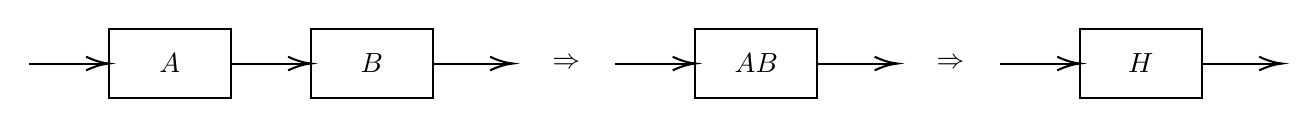
\begin{tikzpicture}[x=0.75pt,y=0.75pt,yscale=-1,xscale=1]
%uncomment if require: \path (0,66.19999694824219); %set diagram left start at 0, and has height of 66.19999694824219

%Shape: Rectangle [id:dp07340500568100361] 
\draw   (67.09,15) -- (125.82,15) -- (125.82,48.56) -- (67.09,48.56) -- cycle ;
%Shape: Rectangle [id:dp9167664477954778] 
\draw   (164.41,15) -- (223.14,15) -- (223.14,48.56) -- (164.41,48.56) -- cycle ;
%Straight Lines [id:da3580760526551523] 
\draw    (125.82,31.78) -- (162.41,31.78) ;
\draw [shift={(164.41,31.78)}, rotate = 180] [color={rgb, 255:red, 0; green, 0; blue, 0 }  ][line width=0.75]    (10.93,-3.29) .. controls (6.95,-1.4) and (3.31,-0.3) .. (0,0) .. controls (3.31,0.3) and (6.95,1.4) .. (10.93,3.29)   ;

%Straight Lines [id:da11851581153449464] 
\draw    (223.14,31.78) -- (259.73,31.78) ;
\draw [shift={(261.73,31.78)}, rotate = 180] [color={rgb, 255:red, 0; green, 0; blue, 0 }  ][line width=0.75]    (10.93,-3.29) .. controls (6.95,-1.4) and (3.31,-0.3) .. (0,0) .. controls (3.31,0.3) and (6.95,1.4) .. (10.93,3.29)   ;

%Straight Lines [id:da8552805925980624] 
\draw    (28.5,31.78) -- (65.09,31.78) ;
\draw [shift={(67.09,31.78)}, rotate = 180] [color={rgb, 255:red, 0; green, 0; blue, 0 }  ][line width=0.75]    (10.93,-3.29) .. controls (6.95,-1.4) and (3.31,-0.3) .. (0,0) .. controls (3.31,0.3) and (6.95,1.4) .. (10.93,3.29)   ;

%Shape: Rectangle [id:dp044934607642187485] 
\draw   (349.69,15) -- (408.42,15) -- (408.42,48.56) -- (349.69,48.56) -- cycle ;
%Straight Lines [id:da7531929098228589] 
\draw    (408.42,31.78) -- (445.01,31.78) ;
\draw [shift={(447.01,31.78)}, rotate = 180] [color={rgb, 255:red, 0; green, 0; blue, 0 }  ][line width=0.75]    (10.93,-3.29) .. controls (6.95,-1.4) and (3.31,-0.3) .. (0,0) .. controls (3.31,0.3) and (6.95,1.4) .. (10.93,3.29)   ;

%Straight Lines [id:da6978811593610801] 
\draw    (311.1,31.78) -- (347.69,31.78) ;
\draw [shift={(349.69,31.78)}, rotate = 180] [color={rgb, 255:red, 0; green, 0; blue, 0 }  ][line width=0.75]    (10.93,-3.29) .. controls (6.95,-1.4) and (3.31,-0.3) .. (0,0) .. controls (3.31,0.3) and (6.95,1.4) .. (10.93,3.29)   ;

%Shape: Rectangle [id:dp06235003242262893] 
\draw   (534.98,15) -- (593.71,15) -- (593.71,48.56) -- (534.98,48.56) -- cycle ;
%Straight Lines [id:da8921643364002274] 
\draw    (593.71,31.78) -- (630.3,31.78) ;
\draw [shift={(632.3,31.78)}, rotate = 180] [color={rgb, 255:red, 0; green, 0; blue, 0 }  ][line width=0.75]    (10.93,-3.29) .. controls (6.95,-1.4) and (3.31,-0.3) .. (0,0) .. controls (3.31,0.3) and (6.95,1.4) .. (10.93,3.29)   ;

%Straight Lines [id:da7745120738778979] 
\draw    (496.39,31.78) -- (532.98,31.78) ;
\draw [shift={(534.98,31.78)}, rotate = 180] [color={rgb, 255:red, 0; green, 0; blue, 0 }  ][line width=0.75]    (10.93,-3.29) .. controls (6.95,-1.4) and (3.31,-0.3) .. (0,0) .. controls (3.31,0.3) and (6.95,1.4) .. (10.93,3.29)   ;


% Text Node
\draw (96.46,31.78) node   {$A$};
% Text Node
\draw (193.77,31.78) node   {$B$};
% Text Node
\draw (379.06,31.78) node   {$AB$};
% Text Node
\draw (287.52,31.78) node   {$\Rightarrow $};
% Text Node
\draw (564.34,31.78) node   {$H$};
% Text Node
\draw (472.59,31.78) node   {$\Rightarrow $};


\end{tikzpicture}
\end{center}

\[ 
	H(j \omega)=A(j \omega)B(j \omega)
 \]
 di conseguenza, visto che usiamo la scala logaritmica, una moltiplicazione diventa una somma: 
 \[ 
	\ln H(j \omega)=\ln A(j \omega) + \ln B(j \omega)
 \]
 
 
 %TODO Questo cos'é? Un altra section? Non so che titolo mettere
 
 Possiamo scrivere $ H(s) $ come:
 \[  
 	K \, \frac{(s-z_1)\,(s-z_2)\,\dots \,(s-z_m)}{(s-p_1)\,(s-p_2)\,\dots \,(s-p_n)}
 \]
 in forma \emph{irriducibile} con $K \in \R  $, $ z_i $ zeri di $ H(s) $ e $ p_i $ poli di $ H(s) $
 
 Possiamo avere tre casi:
 \begin{enumerate}
 	\item $ z_1=0 $ e/o $ p_i = 0 $ cioè poli nell' 
 	\item $ (s-z_i) $ e/o $ (s-p_i) $ non nulli ($ \ne 0  \wedge \in \R$)
 	\item poli complessi coniugati: $ (s-z_i)(s-\overline{z_i}) $ e/o  $ (s-p_i)(s-\overline{p_i}) $
 \end{enumerate}

\subsubsection{Caso 1}
Avremo un termine di questo tipo al denominatore:
 $\displaystyle \frac{1}{s^\nu}  $
con 
\begin{itemize}
	\item $ \nu =0 $ se $ H(s) $ non ha poli o zeri nell'origine
	\item $ \nu >0 $ se $ H(s) $ ha polo nell'origine di molteplicità $ \nu $
	\item $ \nu <0 $ se $ H(s) $ ha zeri nell'origine di molteplicità $\nu$
\end{itemize}

\subsubsection{Caso 2}
Zeri: $ s-z_i \quad z_i \ne 0 $
\[ 
	(s-z_i)=(-z_i)\Big(1+s \frac{1}{-z_1} \Big)=(-z_i)(1+s \tau'_i) \qquad \tau'_i \dot{=} \frac{1}{-z_i}
 \]
 
 (In questo caso $ \tau'_i $ non ha significato fisico) %TODO ho capito bene?
 
 Equivalentemente per i poli: $ s-p_i \quad p_i \ne 0 $
 \[ 
 (s-p_i)=(-z_i)\Big(1+s \frac{1}{-p_1} \Big)=(-p_i)(1+s \tau_i) \qquad \tau_i \dot{=} \frac{1}{-p_i}
 \]
 
 %TODO nei miei appunti è l al posto di e e nell'ultima parte p al posto di Tau, purtroppo non ho trovato sul libro un riferimento 
 (In quest-altro caso, $ \tau_i $, invece, ha significato fisico: la costante di tempo)
 \[ (s-p_i) \rightarrow e^{p_i t} \rightarrow e^{\textstyle -\frac{t}{\tau_1}} \, \text{decadimento esponenziale}\]
 
 \subsubsection{Caso 3}
 
 \[ 
 	(s-z_k)(s-\overline{z_k}) = s^2-z_ks-\overline{z_k}s+z_k \,\overline{z_k} 
 	= s^2 - 2 \Re(z_k) s+\abs{z_k}^2 
 	= \abs{z_k}^2\Big(1-\frac{2 \Re(z_k)}{\abs{z_k}}\frac{s} {\abs{z_k}} + \frac{s^2}{\abs{z_k}^2} \Big)
 \]

 Definiamo $ \omega'_n \dot{=} \abs{z_k} $ come \emph{pulsazione naturale} e $ \zeta_k \dot{=} \frac{-\Re(z_k)}{\abs{z_k}} $ (zeta) come \emph{fattore di smorzamento}, di conseguenza abbiamo: 
 \[ 
 	(s-z_k)(s-\overline{z_k}) = \abs{z_k}^2\Big(1+2\zeta'_k\frac{s}{\omega'_{nk}}+\frac{s^2}{\omega^{'2}_{nk}} \Big)
  \]
  
  Analogamente con $ \omega_n \dot{=} \abs{p_k} $ e $ \zeta_k \dot{=} \frac{-\Re(p_k)}{\abs{p_k}} $ abbiamo:
   \[ 
  (s-p_k)(s-\overline{p_k}) = \abs{p_k}^2\Big(1+2\zeta_k\frac{s}{\omega_{nk}}+\frac{s^2}{\omega^{2}_{nk}} \Big)
  \]
  
  Ora possiamo riscrivere la funzione di trasferimento in $ s $ e in$ j\omega $:
  \[ 
  	H(s) = K_B \, \frac{\prod_i (1+s\tau'_i)^{\mu'_i}\,  \prod_k \Big(1+2\zeta'_k\frac{s}{\omega'_{nk}}+\frac{s^2}{\omega^{'2}_{nk}} \Big)^{\mu'_k}}{s^\nu\, \prod_i (1+s\tau_i)^{\mu_i}\,  \prod_k \Big(1+2\zeta_k\frac{s}{\omega_{nk}}+\frac{s^2}{\omega^{2}_{nk}} \Big)^{\mu_k} }
   \]
     \[ 
   H(j\omega) = K_B \, \frac{\prod_i (1+j\omega\tau'_i)^{\mu'_i}\,  \prod_k \Big(1+j2\zeta'_k\frac{\omega}{\omega'_{nk}}+\frac{\omega^2}{\omega^{'2}_{nk}} \Big)^{\mu'_k}}{(j\omega)^\nu\, \prod_i (1+j\omega\tau_i)^{\mu_i}\,  \prod_k \Big(1+j2\zeta_k\frac{\omega}{\omega_{nk}}+\frac{\omega^2}{\omega^{2}_{nk}} \Big)^{\mu_k} }
   \]
  
\section{Diagrammi base}
   
   Nei diagrammi di Bode posso rappresentare i diagrammi della funzione di trasferimento come combinazione di diagrammi elementari delle varie componenti base :
\[ %TODO-perché tau ha l'indice mentre zeta no?
	K_B \qquad 
	\frac{1}{(j\omega)^\nu} \qquad 
	(1+j\omega\tau_i)^{\mu} \qquad 
	\Big(1+j2\zeta\frac{\omega}{\omega_{n}}+\frac{\omega^2}{\omega^{2}_{n}} \Big)^{\mu}
\]
In cui $ \omega_n > 0 \quad ,\abs{\zeta}<1 \quad,\mu \in \Z $ con $ \mu > 0 \rightarrow$ zeri e $ \mu < 0 \rightarrow$ poli.

\subsection{Termine Costante $ K_B $} 
\[ H(j\omega) = K_B \rightarrow \abs{H(j\omega)}_{dB} = 20 \log \abs{K_B} \]
\begin{figure}[H]
	\centering
	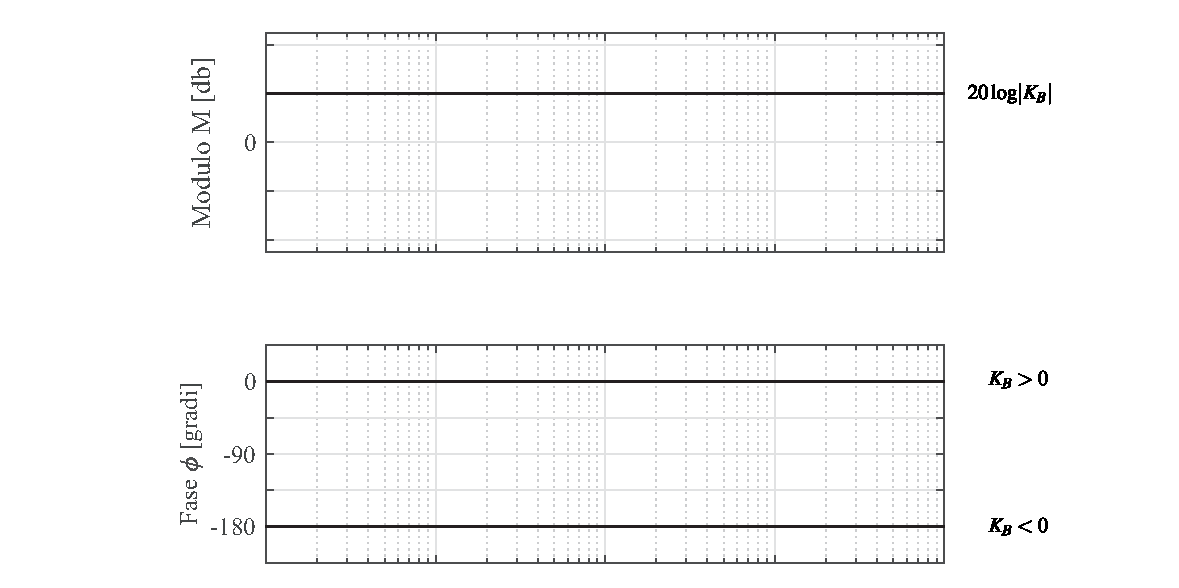
\includegraphics[width=0.8\linewidth]{immagini/cap6_Bode/bodeCost.eps}
	\caption{ Diagramma dell'ampiezza e della fase della costante $  K_B $ }
	\label{fig:bodeCost}
\end{figure}

\subsection{Poli / Zeri in origine}

\begin{gather*}
	H(j\omega) = \frac{1}{(j\omega)^\nu}\\
	\abs{H(j\omega)}_{dB} = 20 \log \Abs{\frac{1}{(j\omega)^\nu}} = 20 ( -\nu) \log \abs{\omega} \qquad \text{dove: }\abs{j\omega}=\abs{\omega}\\
	\arg \bigg(\frac{1}{(j\omega)^\nu}\bigg) = \arg \big((j\omega)^{-\nu}\big) = -\nu \cdot \ang{90} 
\end{gather*}

\begin{figure}[H]
	\centering
	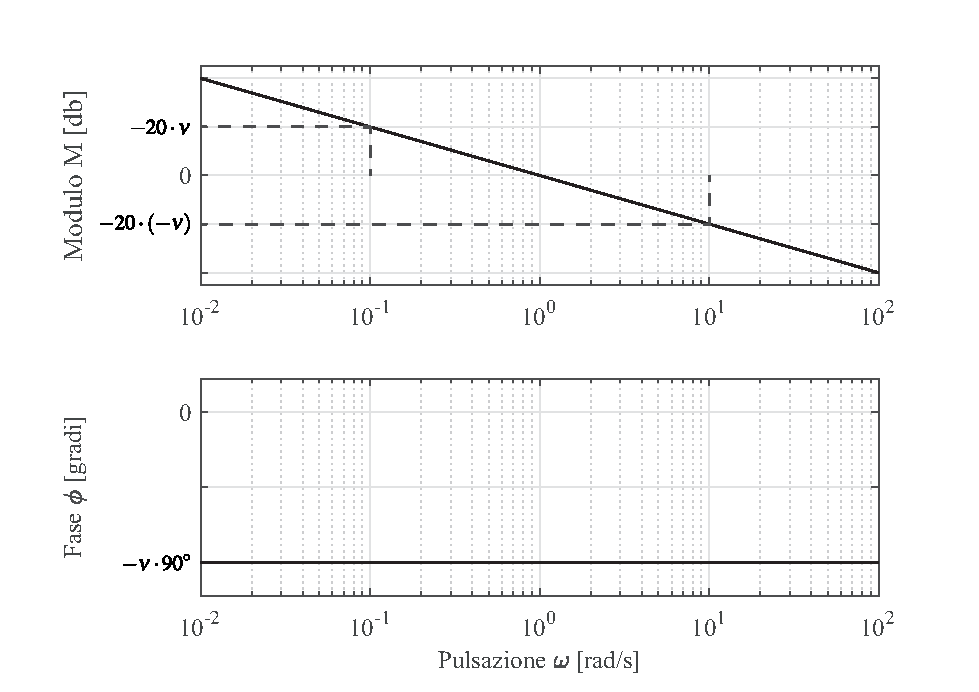
\includegraphics[width=0.8\linewidth]{immagini/cap6_Bode/bodeZPOrig.eps}
	\caption{ Diagramma dell'ampiezza e della fase dei poli e degli zeri in origine}
	\label{fig:bodeZPOrig}
\end{figure}

\begin{nexample}
	\[ H(j\omega) = \frac{1}{(j\omega)^2} \rightarrow \nu = 2 \rightarrow \abs{H(j\omega)}_{dB} = -40 \log \abs{\omega}\]
	\[ \arg \arg \big(H(j\omega)\big) =-\nu \cdot \ang{90} =-2\cdot \ang{90} =\ang{180}  \]
\begin{figure}[H]
	\centering
	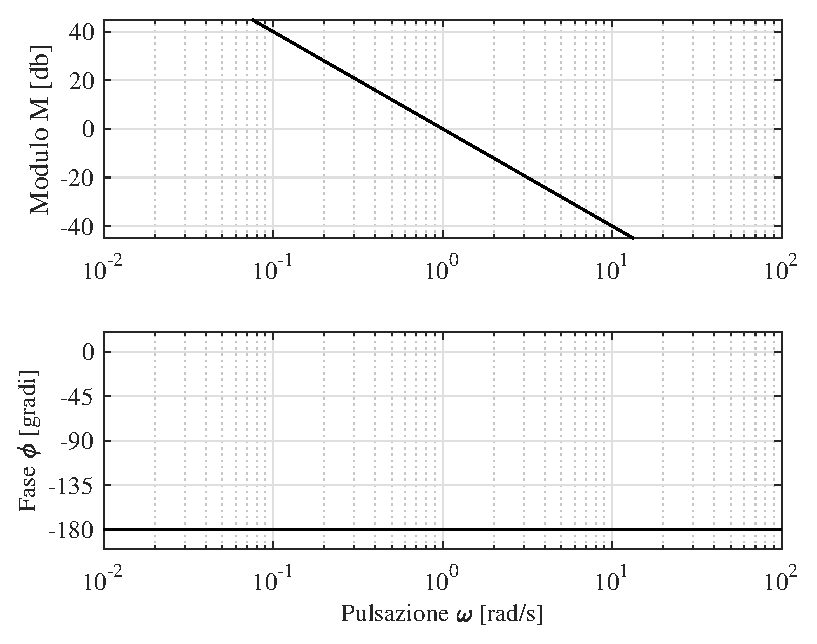
\includegraphics[width=0.7\linewidth]{immagini/cap6_Bode/es1.eps}
	\label{fig:Bode_es1}
\end{figure}
\end{nexample}

\begin{nexample}
	\[ H(j\omega) =j\omega = \frac{1}{(j\omega)^{-1}} \rightarrow \nu = -1 \rightarrow \abs{H(j\omega)}_{dB} = 20 \log \abs{\omega}\]
	\[ \arg \arg \big(H(j\omega)\big) =-\nu \cdot \ang{90} =-(-1)\cdot \ang{90} =\ang{90}  \]
\begin{figure}[H]
	\centering
	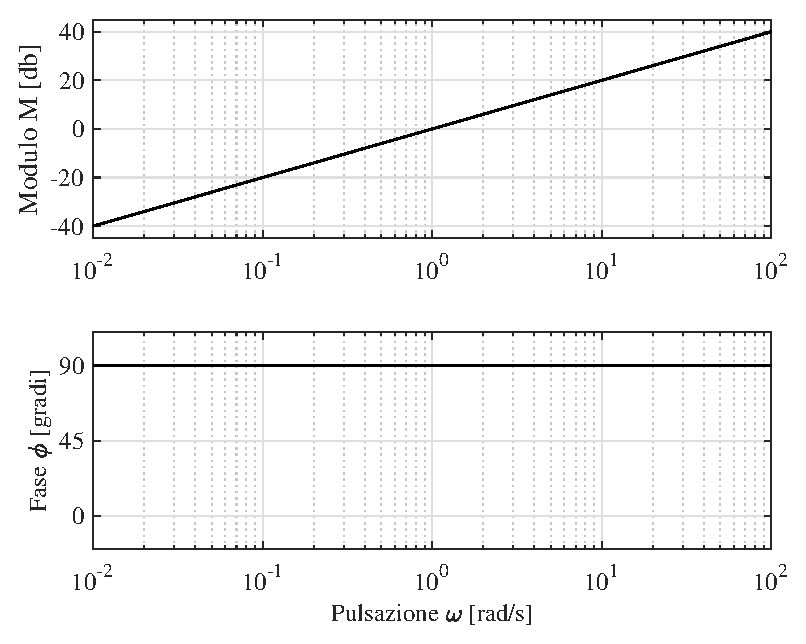
\includegraphics[width=0.7\linewidth]{immagini/cap6_Bode/es2.eps}
	\label{fig:Bode_es2}
\end{figure}
\end{nexample}

\subsection{Termine Binomiale - Poli / Zeri reali}

\[ H(j\omega) = (1+j\omega\tau)^{\mu} \quad \tau \in \R \backslash \{0\} \quad \mu \in \Z \backslash \{0\}  \]
$ \mu>0 $ \emph{Zero Reale} di molteplicità $ \mu $\\
$ \mu<0 $ \emph{Polo Reale} di molteplicità $ -\mu $
\begin{gather*}
	\abs{H(j\omega)}_{dB} = 20 \mu \log \abs{1+j\omega\tau} = 20 \mu \log \sqrt{1+(\omega\tau)^2} \\
	\arg \big(H(j\omega)\big) = \mu \arg(1+j\omega\tau) = \mu \arctan(\omega\tau)
\end{gather*}

Con $ \frac{1}{\abs{\tau}} $ \emph{Pulsazione di Taglio}
\begin{itemize}
	\item $ \abs{\omega\tau} \ll 1 \rightarrow \omega \ll \frac{1}{\abs{\tau}}$
	\item $ \abs{\omega\tau} \gg 1 \rightarrow \omega \gg \frac{1}{\abs{\tau}}$
\end{itemize}

Per l'Ampiezza:
\begin{itemize}
	\item $ \omega \ll \frac{1}{\abs{\tau}} \rightarrow \abs{H(j\omega)}_{dB} \simeq 20\mu \log 1 \simeq 0 $
	\item $ \omega \gg \frac{1}{\abs{\tau}} \rightarrow \abs{H(j\omega)}_{dB} \simeq 20\mu \log \abs{\omega\tau} \simeq 20 \mu \log \abs{\omega} +20 \mu \log \abs{\tau} $
\end{itemize}

Per la Fase:
\begin{itemize}
	\item $ \omega \ll \frac{1}{\abs{\tau}} \rightarrow \arg \big(H(j\omega)\big) \simeq \mu \arg 1 \simeq \ang{0} $ 
	\item $ \omega \gg \frac{1}{\abs{\tau}} \rightarrow \arg \big(H(j\omega)\big) \simeq \mu \arg (j\omega\tau) \simeq \mu \sng(\tau)\ang{90} $ 
\end{itemize}

Viene più facile disegnare la funzione asintotica del segnale rispetto a quella reale.Per l'ampiezza il segnale rimane a $ 0 $ fino alla pulsazione di taglio $ \frac{1}{\abs{\tau}} $ per poi avere una pendenza di $ 20 \mu \dbdec $. La funzione reale, agli estremi, tende a quella asintotica mentre il punto di maggior differenza tra le due è di $ \pm 3 \dbdec $ nella pulsazione di taglio $ \frac{1}{\abs{\tau}} $.
\[ 20\log \abs{1+j\omega\tau} = 20\log \abs{1+j1} = 20\log \sqrt{2} \simeq 3 dB \] 

\begin{figure}[H]
	\centering
	\includegraphics[width=0.7\linewidth]{immagini/cap6_Bode/bodeZPR-Amp.pdf}
	\caption{Grafico per le ampiezze di un zero o polo reale}
	\label{fig:bodezpr-amp}
\end{figure}

Per la fase possiamo approssimare con i punti speciali $ \frac{1}{10\abs{\tau}} $ e $ \frac{10}{\abs{\tau}} $ per l'\emph{approssimazione semplice} oppure con $ \frac{1}{5\abs{\tau}} $ e $ \frac{5}{\abs{\tau}} $ per l'\emph{approssimazione ++} (in quest'ultima l'asisntoto è tangente alla funzione reale).

\begin{figure}[H]
	\centering
	\subfloat[][\emph{ approssimazione semplice}]
	{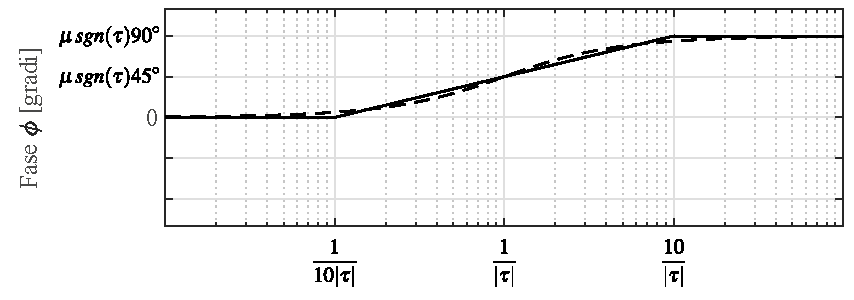
\includegraphics[width=.7\textwidth]{immagini/cap6_Bode/bodeZPR-fas-classica.pdf}} \quad
	\subfloat[][\emph{approssimazione ++}]
	{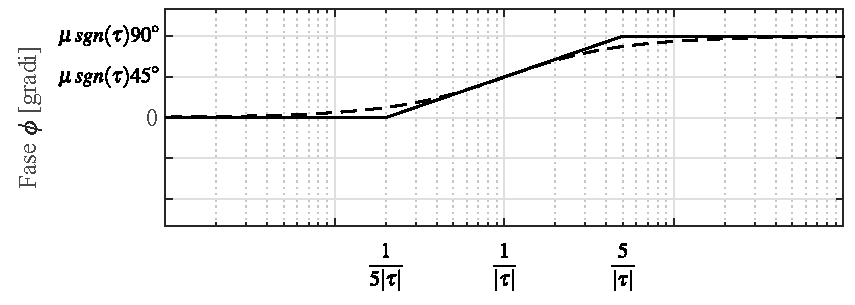
\includegraphics[width=.7\textwidth]{immagini/cap6_Bode/bodeZPR-fas-++.pdf}} 
	\caption{ Grafico della fase di un zero o polo reale. }
	\label{fig:bodezpr-fas}
\end{figure}

\begin{nexample}
	\[ H(j\omega) = 1-j\omega2 \qquad\tau<0, \, \mu = 1 \]
\begin{figure}[H]
	\centering
	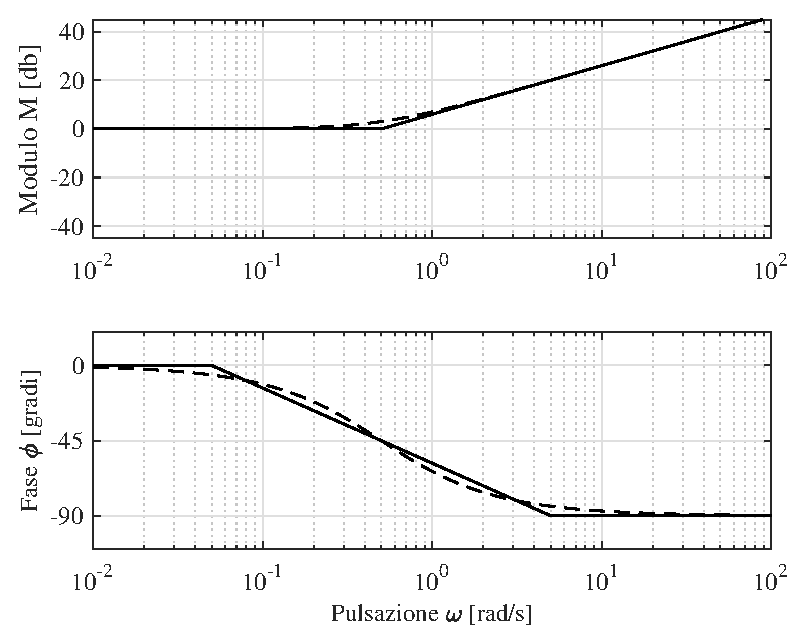
\includegraphics[width=0.7\linewidth]{immagini/cap6_Bode/es3.eps}
	\label{fig:Bode_es3}
\end{figure}	
\end{nexample}

\begin{nexample}
	\[ H(j\omega) = \frac{1}{1-j\omega2} = (1-j\omega2)^2 \qquad\tau = 2, \, \mu = -1 \]
	%TODO controlla elevato alla 2?
\begin{figure}[H]
	\centering
	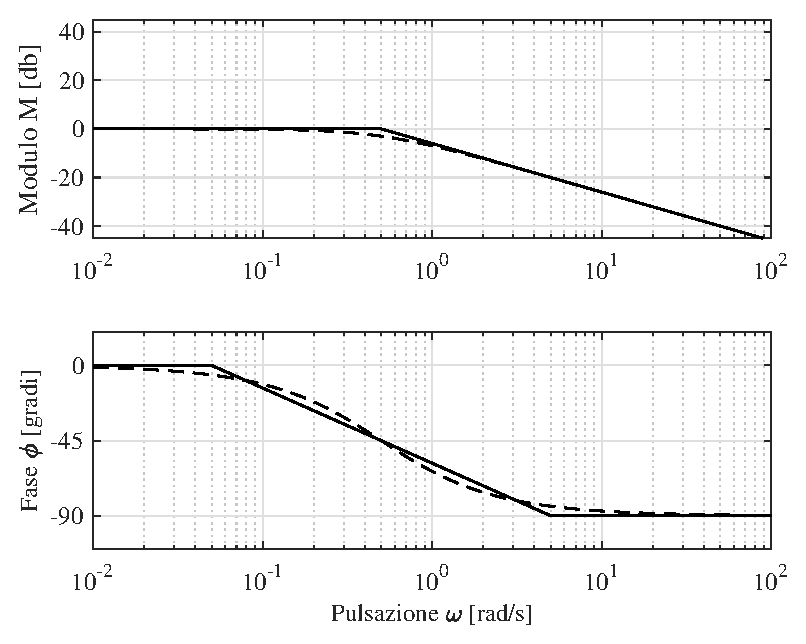
\includegraphics[width=0.7\linewidth]{immagini/cap6_Bode/es4.eps}
	\label{fig:Bode_es4}
\end{figure}	
\end{nexample}

\subsection{Termine Trinomio}
\begin{gather*}
	\Big(1+j2\zeta\frac{\omega}{\omega_{n}}-\frac{\omega^2}{\omega^{2}_{n}} \Big)^{\mu}\\
	\abs{H(j\omega)}_{dB} = 20 \mu \log \Abs{\underbrace{1-\frac{\omega^2}{\omega^{2}_{n}}}_{\text{\scriptsize Parte Reale}}+\underbrace{j2\zeta\frac{\omega}{\omega_{n}}}_{\text{\scriptsize Parte Immaginaria}}} = 20\mu \log \sqrt{\bigg(1-\frac{\omega^2}{\omega^{2}_{n}} \bigg)^2+\bigg(j2\zeta\frac{\omega}{\omega_{n}}\bigg)^2}\\
	\arg\big(H(j\omega)\big) = \arg(a+jb) = 
	\begin{cases}
		\arctan\big(\frac{b}{a}\big) & ,a>0\\
		\sng(b)\frac{\pi}{2} & ,a=0,\, b \ne 0\\
		\arctan\big(\frac{b}{a}\big) + \sng(b)\pi & ,a<0,\, b \ne 0 
	\end{cases} 
\end{gather*}

Studiamo i vari casi:
\[ 
	1-\frac{\omega^2}{\omega^{2}_{n}}>0 \rightarrow \frac{\omega^2}{\omega^{2}_{n}} <1 \rightarrow \omega^2 < \omega^2_n \rightarrow 
	\begin{cases}
		\omega < \omega_n &a>0\\
		\omega > \omega_n &a<0\\
		\omega = \omega_n &a=0
	\end{cases}
\]

Quindi:
\[ 
 	\arg\big(H(j\omega)\big) = 
 	\begin{cases}
	 	\arctan\Bigg(\frac{2\zeta\frac{\omega}{\omega_n}}{1-\frac{\omega^2}{\omega^{2}_{n}}}\Bigg) & \omega < \omega_n\\
	 	\sng(\zeta)\frac{\pi}{2} &	\omega = \omega_n\\
	 	\arctan\Bigg(\frac{2\zeta\frac{\omega}{\omega_n}}{1-\frac{\omega^2}{\omega^{2}_{n}}}\Bigg)+ \sng(\zeta)\pi & \omega > \omega_n\\
 	\end{cases}
\]
  
Guardiamo ora l'ampiezza. Anche qui calcoliamo il segnale asintotico:
\begin{gather*}
  	\omega \ll \omega_n \rightarrow \abs{H(j\omega)}_{dB}\simeq 20\mu \log(1) = 0\\
  	\omega \gg \omega_n \rightarrow \abs{H(j\omega)}_{dB}\simeq 20\mu \sqrt{	\bigg(\frac{\omega^2}{\omega^2_n}\bigg)^2} = 40\mu \log(\omega)-40 \mu \log(\omega_n)
\end{gather*}

\begin{figure}[H]
	\centering
	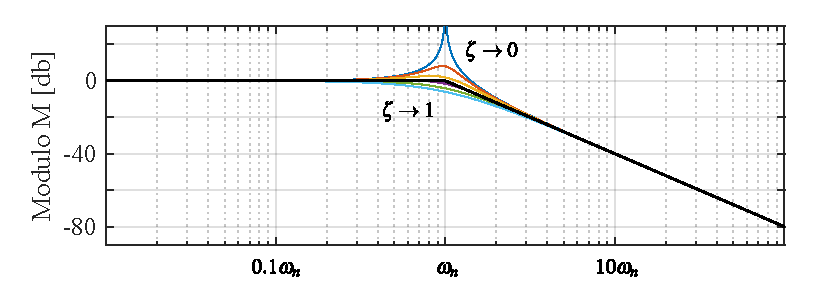
\includegraphics[width=0.8\linewidth]{immagini/cap6_Bode/bodeBin-amp.pdf}
	\caption{Grafico dell'Ampiezza di un termine binomio, la parte reale è al variare di $ \zeta $}
	\label{fig:bodeBin-Amp}
\end{figure}

Guardiamo adesso la fase:
\begin{equation*}
	\omega \ll \omega_n \rightarrow \arg \big(H(j\omega)\big) = \arg(1)
\end{equation*}
\begin{multline*}
	\omega \gg \omega_n \rightarrow \arg \big(H(j\omega)\big) = \mu \Bigg(\arctan\Bigg(\overbrace{\frac{2\zeta\frac{\omega}{\omega_n}}{1-\frac{\omega^2}{\omega^{2}_{n}}}}^{\parbox{7
			em}{\scriptsize Il denominatore tende a infinito prima del numeratore quindi tende a 0}}\Bigg)+ \sng(\zeta)\pi\Bigg) \\= \mu \arctan(0) + \mu \sng(\zeta)\pi = \mu \sng(\zeta)\pi
\end{multline*}

\begin{figure}[H]
	\centering
	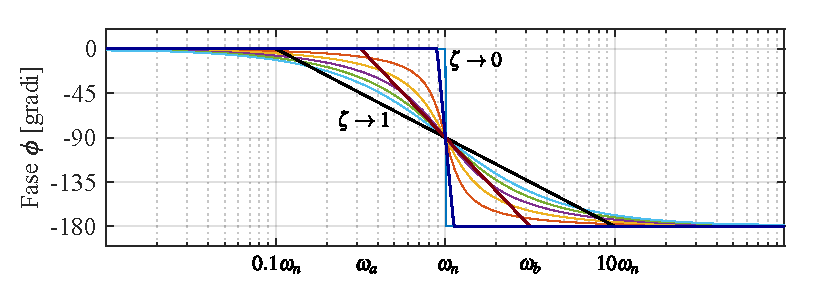
\includegraphics[width=0.8\linewidth]{immagini/cap6_Bode/bodeBin-fas.pdf}
	\caption{Grafico della fase di un termine binomio al variare di $ \zeta $}
	\label{fig:bodeBin-Fas}
\end{figure}
dove: $\displaystyle \omega_a \simeq \frac{1}{5^{\abs{\zeta}}}\omega_n \qquad \omega_b \simeq 5^{\abs{\zeta}}\omega_n$


	Con $\displaystyle \abs{\zeta}=1 \rightarrow \zeta =\frac{\Re (Z_K)}{\abs{Z_K}} \equiv \Big(1+\sng(\zeta)j \omega \frac{1}{\omega_n}\Big)^{2\mu} $. 	
	In questo caso la differenza tra reale e asintotico è di $ 6 dB $
	
	Con $ \displaystyle \abs{\zeta} = 0 \rightarrow H(j\omega) = \Big(1-\frac{\omega^2}{\omega2_n}\Big)^\mu $.
	Abbiamo, quindi, 2 poli complessi coniugati con $ \Re =0 $ (completamente immaginari). Di conseguenza:
	\begin{gather*}
		H(j\omega)=
		\begin{cases}
			20\mu \log(1)=0 &\omega \ll \omega_n\\
			40\mu\log\big(\frac{\omega}{\omega_n}\big) &\omega \gg \omega_n
		\end{cases}\\
		\arg \big(H(j\omega)\big) = 
		\begin{cases}
			0 &\omega \ll \omega_n\\
			\pm \mu \ang{180} &\omega \gg \omega_n
		\end{cases}
	\end{gather*}
Si può scegliere come convenzione se fare + o - \ang{180}, noi useremo +\ang{180}.

Per comodità, negli esercizi si vuole approssimare la funzione reale. È bene precisare dove la funzione reale si trova, in confronto a quella asintotica, sul punto $ \omega_n $:
\begin{align*}
	0<\abs{\zeta}<\frac{1}{2} &\rightarrow \, \text{interseca l'asse delle ascisse a destra di $ \omega_n $}
		\begin{cases}
			\text{sotto a }\omega_n &,\mu >0\\
			\text{sopra a }\omega_n &,\mu <0
		\end{cases}\\
	\abs{\zeta} =\frac{1}{2} &\rightarrow\, \text{passa per $ \omega_n $}\\
	\frac{1}{2}<\abs{\zeta}<\frac{\sqrt{2}}{2} &\rightarrow \, \text{interseca l'asse delle ascisse a sinistra di $ \omega_n $}\\
	\frac{\sqrt{2}}{2}<\abs{\zeta}<1 &\rightarrow \,
		\begin{cases}
			\text{sopra a }\omega_n &,\mu >0\\
			\text{sotto a }\omega_n &,\mu <0
		\end{cases}
\end{align*}



\section{Esempi di esercizi}
\begin{nexample}
	\[ H(s) = \frac{\overbrace{10}^{K} \, (s+1)}{(s+0,1)\,(s-1)} \]
	Trasformiamo:
	\begin{gather*}
		s+1\rightarrow z_1 =-1\rightarrow\tau'_1 = \frac{1}{-z_1}= \frac{1}{-(-1)}=1 \quad \mu'_1 = 1 \\
		s+0,1\rightarrow p_1 =-0,1\rightarrow\tau_1 = \frac{1}{-p_1} = \frac{1}{-(-0,1)}=10 \quad \mu_1 = -1 \\
		s-1\rightarrow p_2 =-0,1\rightarrow\tau_1 = \frac{1}{-p_2}= \frac{1}{-1}=-1 \quad \mu_2 = -1 \\
	\end{gather*}
	%TODO non é -100?
	\[
		H(s) = \frac{10\overbrace{(+1)}^{-z_1} \, (1+s\tau'_1)}{\underbrace{(+0,1)}_{-p_1}(1+s\tau_1)\,\underbrace{(-1)}_{-p_2}(1+s\tau_2)} =
		\frac{100 \, (1+s\tau'_1)}{(1+s\tau_1)\,(1+s\tau_2)} = 
		\frac{100 \, (1+s)}{(1+10s)\,(1-s)} 
	\]
	In forma di Bode:
	\[  H(j\omega) = \frac{100 \, (1+j\omega\tau'_1)}{(1+j\omega\tau_1)\,(1+j\omega\tau_2)}\]
	
%\begin{figure}[H]
%	\centering
%	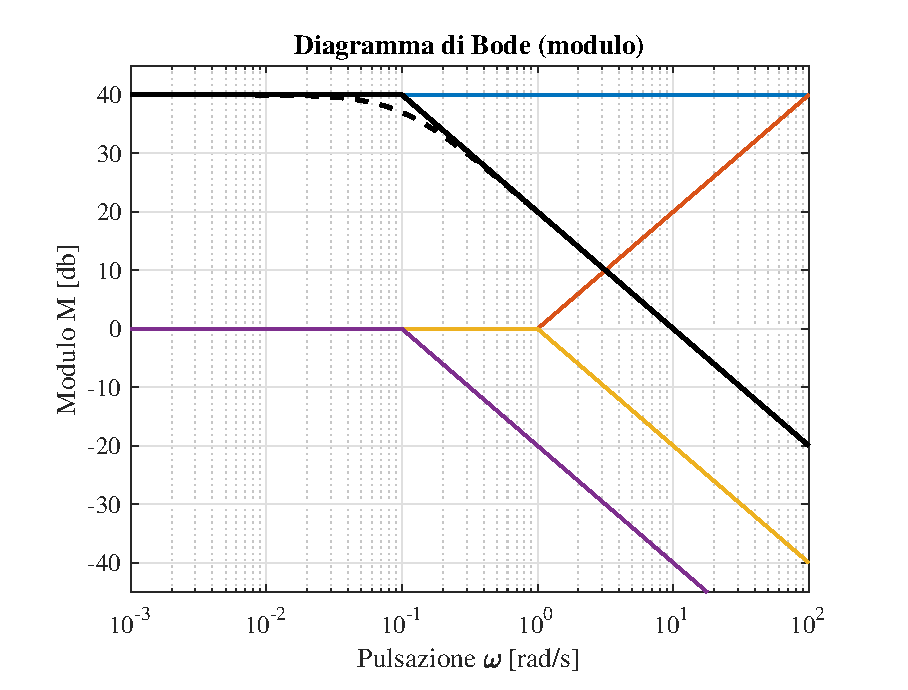
\includegraphics[width=0.7\linewidth]{immagini/cap6_Bode/es5-amp.eps}
%	\caption{Diagramma totale delle ampiezze, la risultante è la somma di tutti i diagrammi base}
%	\label{fig:es5-amp}
%\end{figure}
%\begin{figure}[H]
%	\centering
%	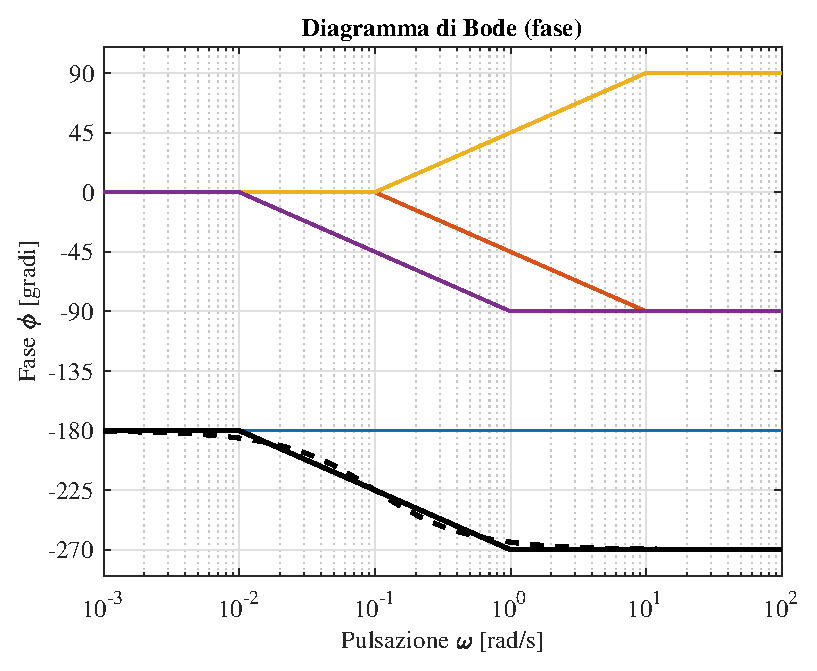
\includegraphics[width=0.7\linewidth]{immagini/cap6_Bode/es5-fas.eps}
%	\caption{Diagramma totale delle fasi, la risultante è la somma di tutti i diagrammi base}
%	\label{fig:es5-fas}
%\end{figure}

\begin{figure}[H]
	\centering
	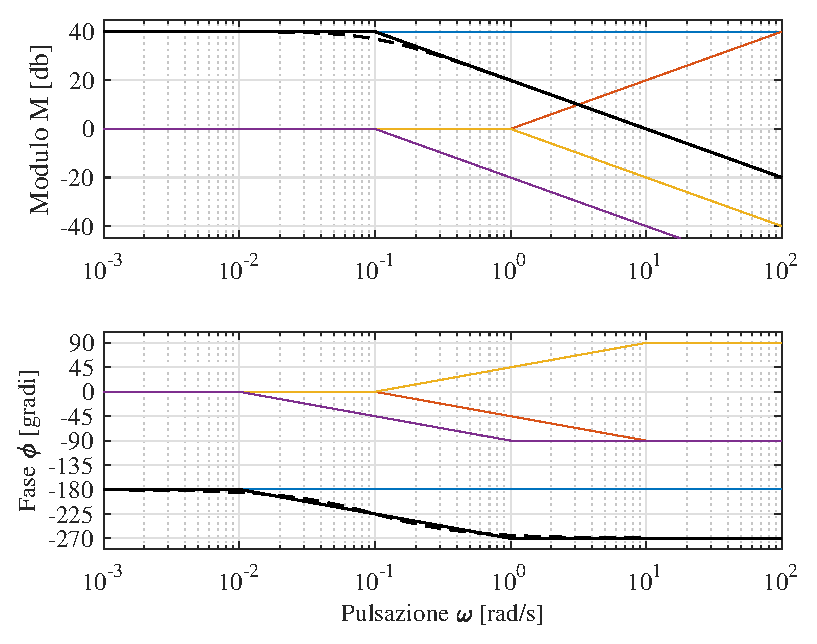
\includegraphics[width=0.7\linewidth]{immagini/cap6_Bode/es5.eps}
	\caption{Diagramma totale delle ampiezze e delle fasi, la risultante è la somma di tutti i diagrammi base}
	\label{fig:es5}
\end{figure}

\end{nexample}





